\documentclass[aspectratio=169]{beamer}
\usepackage{lmodern}
%\usetheme{Madrid}
%\usecolortheme{giantoak}
\newcommand*\oldmacro{}
\let\oldmacro\insertshorttitle
\renewcommand*\insertshorttitle{\oldmacro\hfill\insertframenumber\,/\,\inserttotalframenumber}
\usepackage[framemethod=tikz]{mdframed}

%\usepackage{beamerthemesplit}
\usepackage{textpos}
\usepackage{pgf}
\usepackage{ulem}
%\logo{\pgfputat{\pgfxy(0,-.4)}{\pgfbox[right,base]{\includegraphics[height=1.0cm]{logo.jpg}}}}
%\newcommand{\nologo}{\setbeamertemplate{logo}{}}
\usepackage{booktabs}
\usepackage{graphicx}
\theoremstyle{principle}
\newtheorem*{principle}{Design Principle}


\titlegraphic{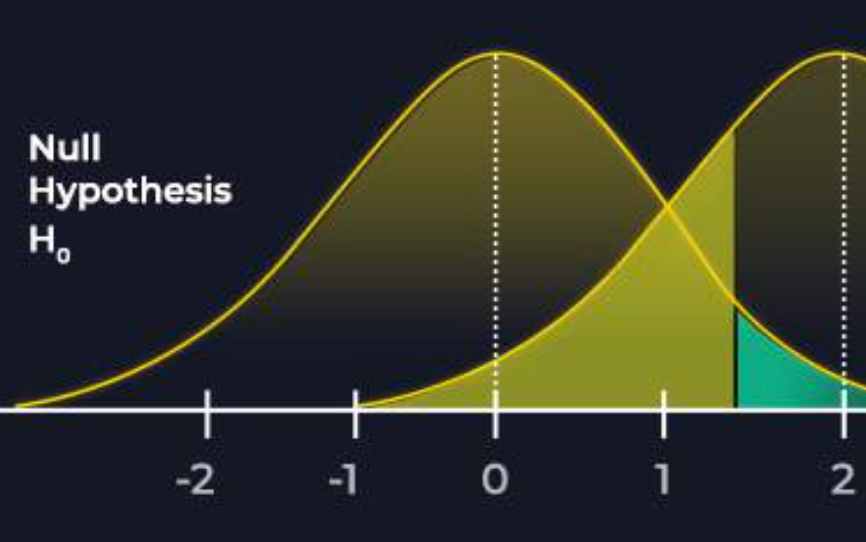
\includegraphics[width=1.0\paperwidth]{distros.png}}

\title{Amendments}
%\author[Jeremy Kedziora]{Wind Data Science Team\\
%\small{Uptake}}
\date{}

\begin{document}

%{
%%\nologo
%\begin{frame}
%    \maketitle
%\end{frame}
%}
%pages 1-7, 8-9, 14-15.


{
%  \usebackgroundtemplate{
\includegraphics[width=1.0\paperwidth]{statistics-review.jpg}}
  \usebackgroundtemplate{
\includegraphics[scale=0.127]{catch_and_release.jpg}}
  \begin{frame}[plain]
  
\begin{mdframed}[tikzsetting={draw=white,fill=white,fill opacity=0.6,draw opacity=0.4,
               line width=0pt},backgroundcolor=none,leftmargin=20,
               rightmargin=20,innertopmargin=4pt]
\begin{center}
\Huge \textbf{The Bootstrap}
\end{center}
\end{mdframed}

  \end{frame}
}

%most reliant on human cognition
%limited only by cognition
%hypothesis generating scheme often functioning as a gateway into more statistical analysis

%%@@@@@@@@@@@@@@@@@@@@@@@@@@@@@@@@@@@@@@@@@@@@@@@@@
%\begin{frame}
%\frametitle{Napoleon's Progress}
%\begin{center}
%
\includegraphics[scale=0.4]{experiment.png}
%
\includegraphics[scale=0.35]{stars.png}
%\end{center}
%
%\end{frame}

%@@@@@@@@@@@@@@@@@@@@@@@@@@@@@@@@@@@@@@@@@@@@@@@@@
\begin{frame}
\frametitle{Today:}

\begin{itemize}
\item Introduce bootstrapping;
\bigskip
\bigskip
\bigskip

\item Talk about confidence intervals (the most common application of the bootstrap);
\bigskip
\bigskip
\bigskip

\item Examples!


\end{itemize}

\end{frame}

%@@@@@@@@@@@@@@@@@@@@@@@@@@@@@@@@@@@@@@@@@@@@@@@@@
\begin{frame}
\frametitle{Recall sampling: Definitions}
\begin{itemize}
\item \textbf{Population}: a `complete' group of $N$ objects, items, entities, or events of interest -- e.g. all adults living in the US;
\bigskip
\item \textbf{Sample}: a selected subset of $n$ individuals from a population -- e.g. 5,000 US adults appearing in a poll;
\bigskip
\item \textbf{Summary Statistic}: a summary of the information in a set of observations -- e.g. mean, median, mode, etc.;
\bigskip
\item \textbf{Census}: a counting of all elements of the population;
\bigskip
\item \textbf{Sampling}: the act of collecting a sample of size $n$ from a population of size $N$;
\begin{itemize} 
\item sample only when we can’t perform a census;
\item typically the sample size $n<<N$;
\end{itemize}
\bigskip
\item \textbf{Sample Statistic}: a summary statistic computed from a sample that estimates the unknown population parameter.
\end{itemize}
\end{frame}

%@@@@@@@@@@@@@@@@@@@@@@@@@@@@@@@@@@@@@@@@@@@@@@@@@
\begin{frame}
\frametitle{Recall sampling: A simple example -- marbles in a bag}

\begin{itemize}
\item Consider a bag full of marbles;
\begin{itemize}
\item the number of marbles in the bag is unknown;
\item there are multiple but unknown colors of marbles in the bag;
\item the fraction of any particular color of marbles in the bag is unknown;
\end{itemize}
\bigskip
\item Questions we could ask:
\begin{itemize}
\item How many marbles are in the bag?
\item How many colors of marbles are in the bag?
\item \textbf{What is the fraction of blue marbles in the bag?}
\end{itemize}
\bigskip
\item Assume we can't just dump the bag out or remove marbles from it permanently -- can we devise a process to answer any of these questions?
\bigskip
\item What about the following:
\begin{enumerate}
\item Stick a hand in the top of the bag and pull out handful of marbles;
\item Observe them;
\item Return them to the bag and then mix;
\item Repeat.
\end{enumerate} 
\end{itemize}

\end{frame}

%@@@@@@@@@@@@@@@@@@@@@@@@@@@@@@@@@@@@@@@@@@@@@@@@@
\begin{frame}
\frametitle{\textbf{Bootstrapping} is REALLY similar to this!}
\begin{center}
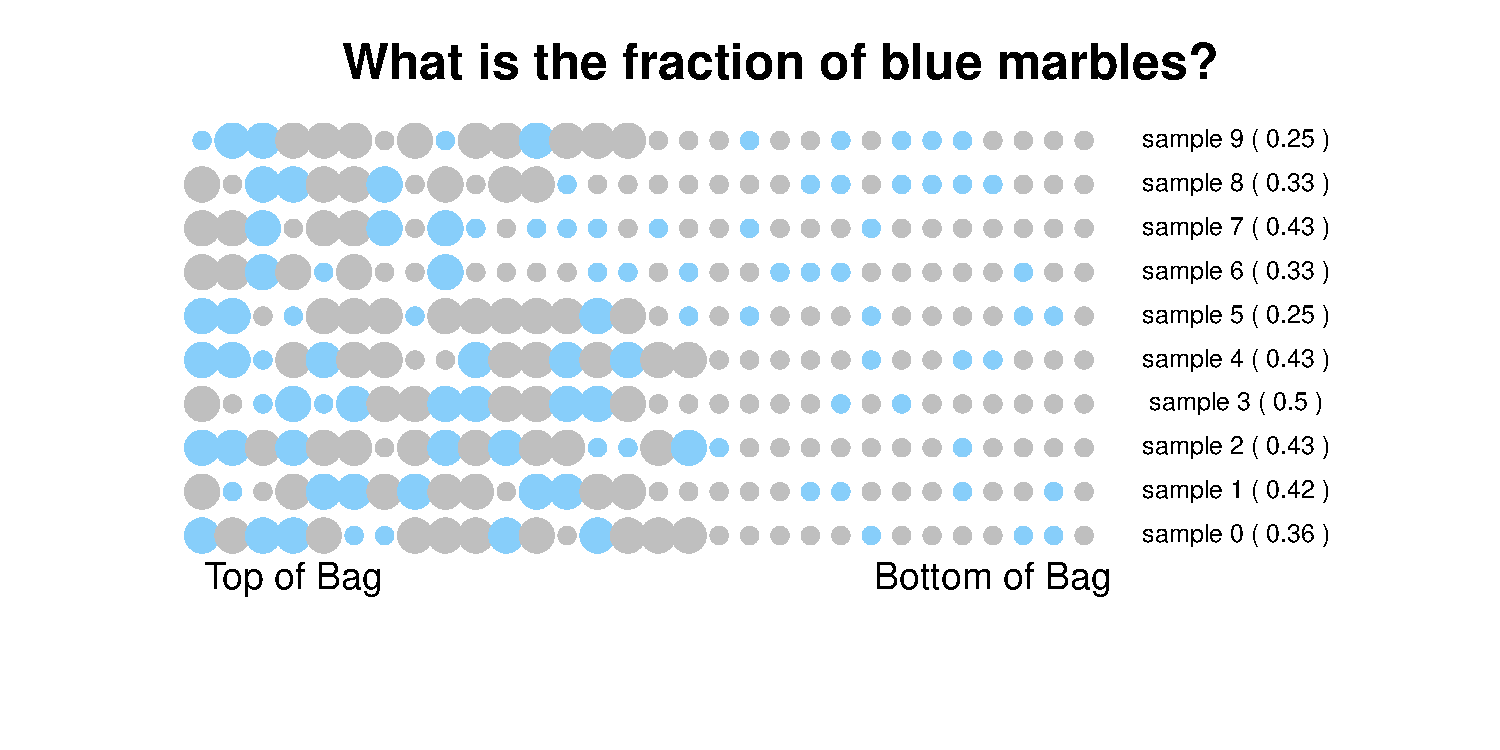
\includegraphics[scale=0.57]{sample_full.pdf}
\end{center}
\end{frame}

%@@@@@@@@@@@@@@@@@@@@@@@@@@@@@@@@@@@@@@@@@@@@@@@@@
\begin{frame}
\frametitle{What is bootstrapping?}

\begin{itemize}
\item Let's return to the marbles in a bag experiment with a slight modification -- suppose we know there are 30 marbles and we want to know the fraction of blue marbles;
\begin{enumerate}
\item Sample marbles \textbf{with replacement}:
\begin{enumerate}
\item Stick a hand in the bag and pull out a marble;
\item Observe whether it is blue; 
\item Return it to the bag and mix; 
\item Repeat this 30 times -- these 30 observations will be one bootstrap sample;
\end{enumerate}
\item Compute the fraction of blue marbles you observed in your bootstrap sample;
\item Repeat steps 1 and 2 many (1000s of) times.
\end{enumerate} 

\bigskip

\item This is all bootstrapping is -- sample from your data with replacement, compute the statistic you are interested in, repeat!

\end{itemize}

\end{frame}

%@@@@@@@@@@@@@@@@@@@@@@@@@@@@@@@@@@@@@@@@@@@@@@@@@
\begin{frame}
\frametitle{Confidence Intervals -- most common application of bootstrapping!}

\begin{itemize}
\item We'd like to measure the variation of a statistic (e.g. the $\beta$s in a regression);
\begin{itemize}
\item Want to be able to say: `effect of x on y is $\beta \pm z$;
\item Typical way to do this is to use a \textbf{confidence interval};
\end{itemize}
\bigskip

\item A 95\% confidence interval is a region around the statistic, a plus/minus:
\begin{itemize}
\item \textbf{Interpretation 1}: there is a 95\% probability that the 95\% confidence interval calculated using a future sample will include the true population parameter;
\item \textbf{Interpretation 2}: the region contains values that are not statistically significantly different from the point estimate at the 0.05 level;
\end{itemize}
\bigskip

\item Rough rules of thumb:
\begin{itemize}
\item The 95\% confidence interval is twice the standard error;
\item If the 95\% confidence interval does not include 0 then we reject the null of no effect.
\end{itemize}

\end{itemize}

% latex table generated in R 4.1.1 by xtable 1.8-4 package
% Mon Nov 21 09:57:48 2022
\begin{table}[ht]
\centering
\begin{tabular}{rrrrr}
  \hline
 & Estimate & Std. Error & t value & Pr($>$$|$t$|$) \\ 
  \hline
(Intercept) & 1.3127 & 1.0125 & 1.30 & 0.1963 \\ 
  percent & 0.0428 & 0.0188 & 2.28 & 0.0237 \\ 
   \hline
\end{tabular}
\end{table}

\end{frame}

%@@@@@@@@@@@@@@@@@@@@@@@@@@@@@@@@@@@@@@@@@@@@@@@@@
\begin{frame}
\frametitle{Using Bootstrapping to Estimate Confidence Intervals}

\begin{itemize}
\item Three steps:
\begin{enumerate}
\item Sample from the original data (or bag of marbles) with replacement and compute the stat of interest 1000 times;
\item Sort the results from smallest to largest; 
\item Take the 25th and 975th results from this sorted list -- these are the boundaries of your confidence interval;
\end{enumerate}
\bigskip

\item But we have other ways of thinking about the error in our inferences (e.g. p-values) so why do this?
\begin{itemize}
\item[]\color{white} Some statistics do not have things like $p$-values that are computable using equations (e.g. medians,  model performance metrics);
\item[]\color{white} Some problems in regression will compromise the $p$-value but we can easily get a sense of whether to reject the null with bootstrapped CIs.
\end{itemize}
\end{itemize}

\end{frame}

%@@@@@@@@@@@@@@@@@@@@@@@@@@@@@@@@@@@@@@@@@@@@@@@@@
\begin{frame}
\frametitle{Using Bootstrapping to Estimate Confidence Intervals}

\begin{itemize}
\item Three steps:
\begin{enumerate}
\item Sample from the original data (or bag of marbles) with replacement and compute the stat of interest 1000 times;
\item Sort the results from smallest to largest; 
\item Take the 25th and 975th results from this sorted list -- these are the boundaries of your confidence interval;
\end{enumerate}
\bigskip

\item But we have other ways of thinking about the error in our inferences (e.g. p-values) so why do this?
\begin{itemize}
\item Some statistics do not have things like $p$-values that are computable using equations (e.g. medians, model performance metrics);
\item[]\color{white} Some problems in regression will compromise the $p$-value but we can easily get a sense of whether to reject the null with bootstrapped CIs.
\end{itemize}
\end{itemize}

\end{frame}

%@@@@@@@@@@@@@@@@@@@@@@@@@@@@@@@@@@@@@@@@@@@@@@@@@
\begin{frame}
\frametitle{Using Bootstrapping to Estimate Confidence Intervals}

\begin{itemize}
\item Three steps:
\begin{enumerate}
\item Sample from the original data (or bag of marbles) with replacement and compute the stat of interest 1000 times;
\item Sort the results from smallest to largest; 
\item Take the 25th and 975th results from this sorted list -- these are the boundaries of your confidence interval;
\end{enumerate}
\bigskip

\item But we have other ways of thinking about the error in our inferences (e.g. p-values) so why do this?
\begin{itemize}
\item Some statistics do not have things like $p$-values that are computable using equations (e.g. medians, model performance metrics);
\item Some problems in regression will compromise the $p$-value but we can easily get a sense of whether to reject the null with bootstrapped CIs.
\end{itemize}
\end{itemize}

\end{frame}

%@@@@@@@@@@@@@@@@@@@@@@@@@@@@@@@@@@@@@@@@@@@@@@@@@
\begin{frame}
\frametitle{Step 1: sample w/ replacement from the marble bag 1000 times}

\begin{center}
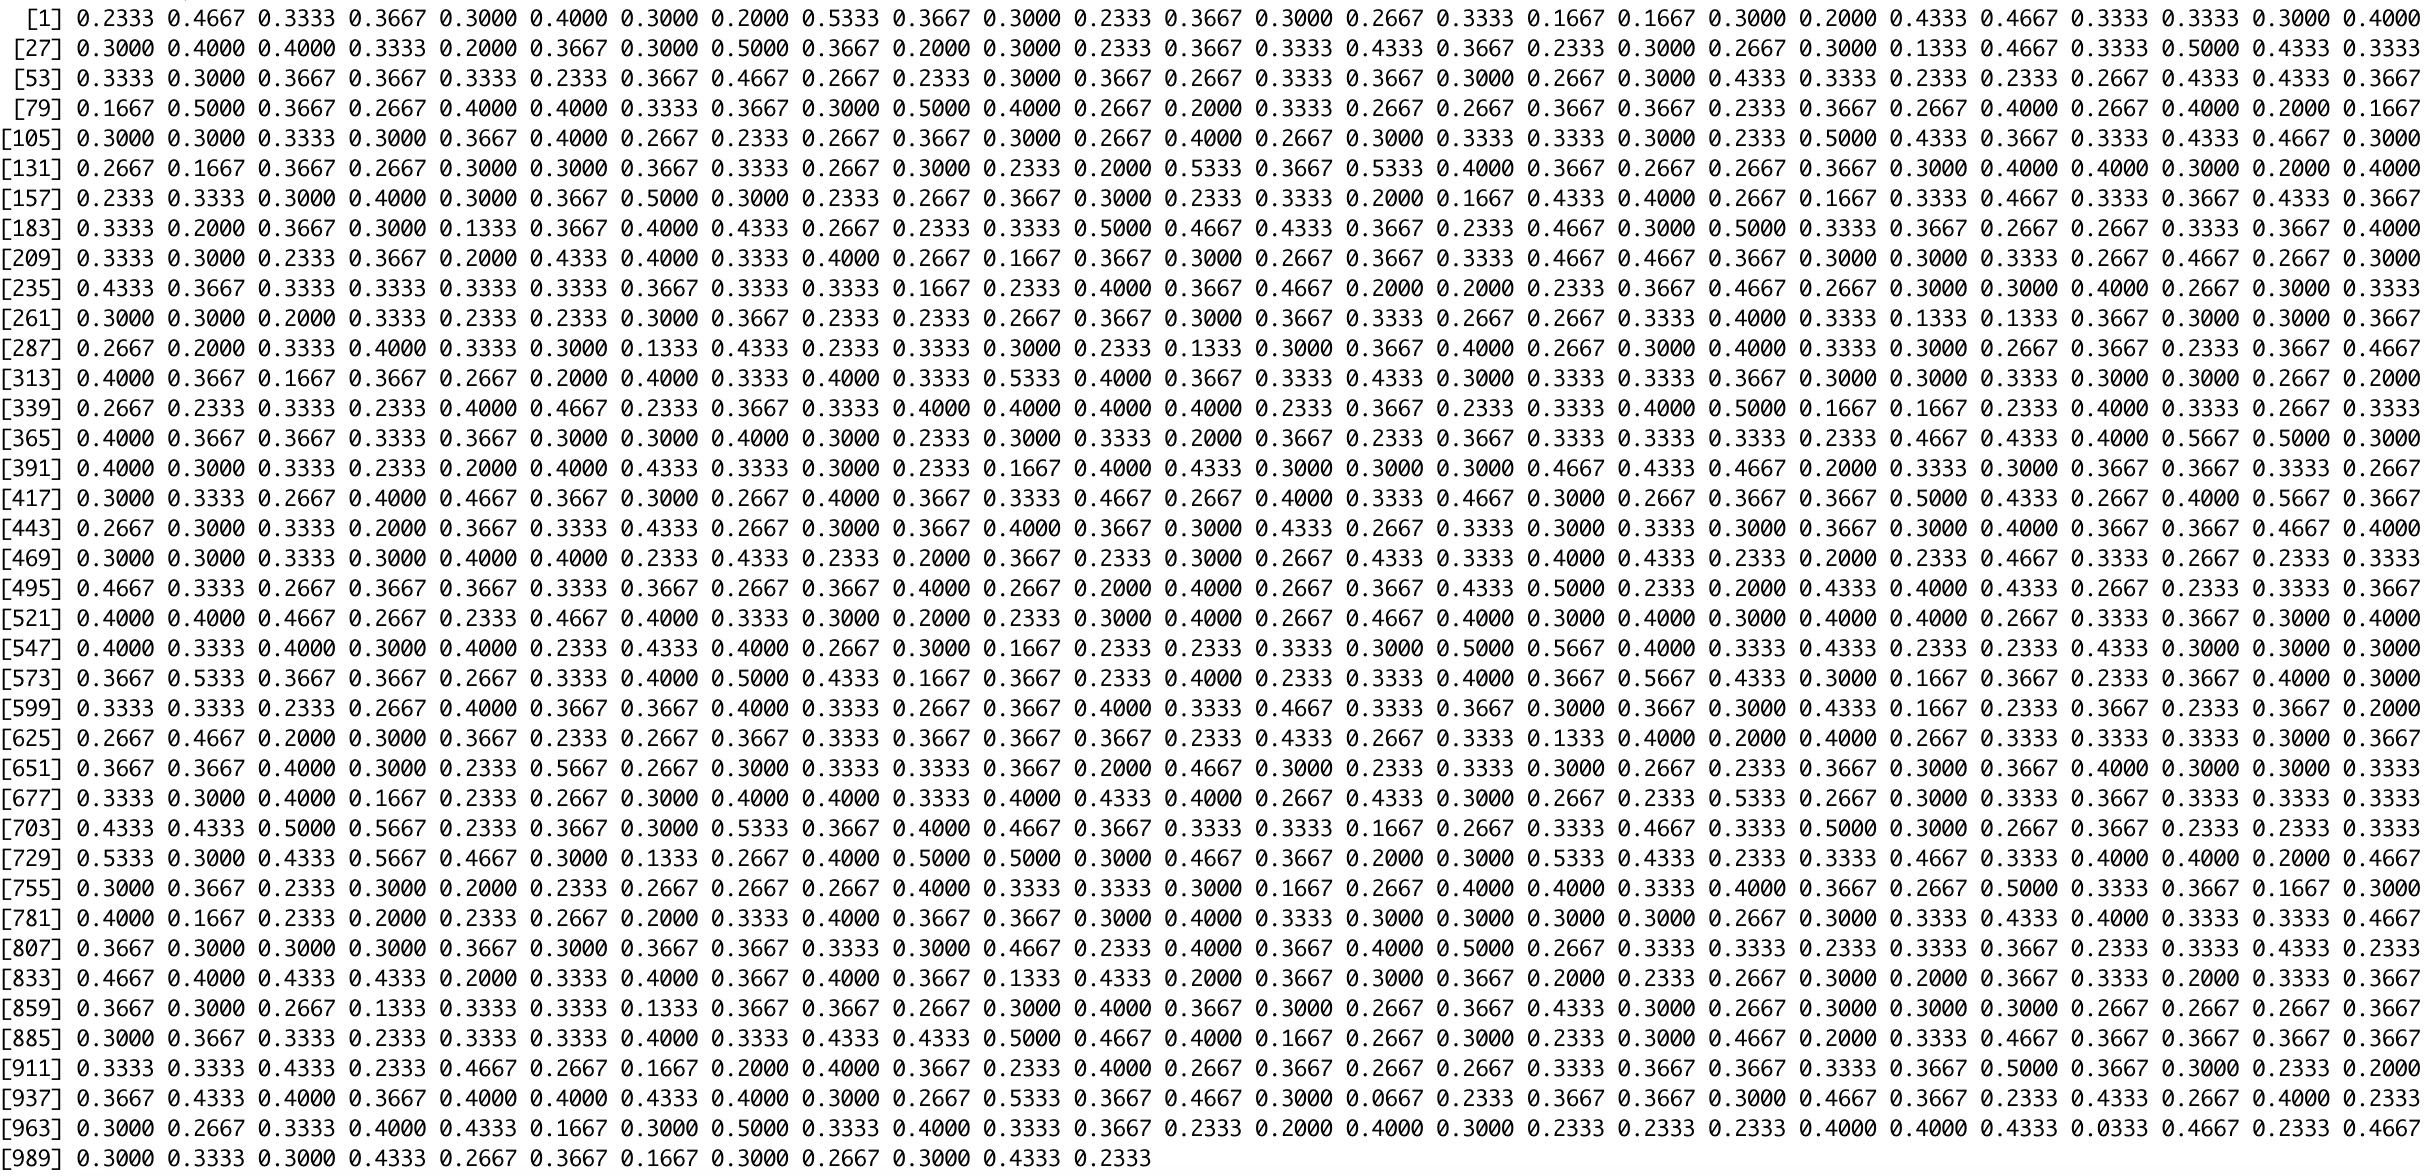
\includegraphics[scale=0.33]{numbers.png}
\end{center}

\end{frame}

%@@@@@@@@@@@@@@@@@@@@@@@@@@@@@@@@@@@@@@@@@@@@@@@@@
\begin{frame}
\frametitle{Step 2: sort}

\begin{center}
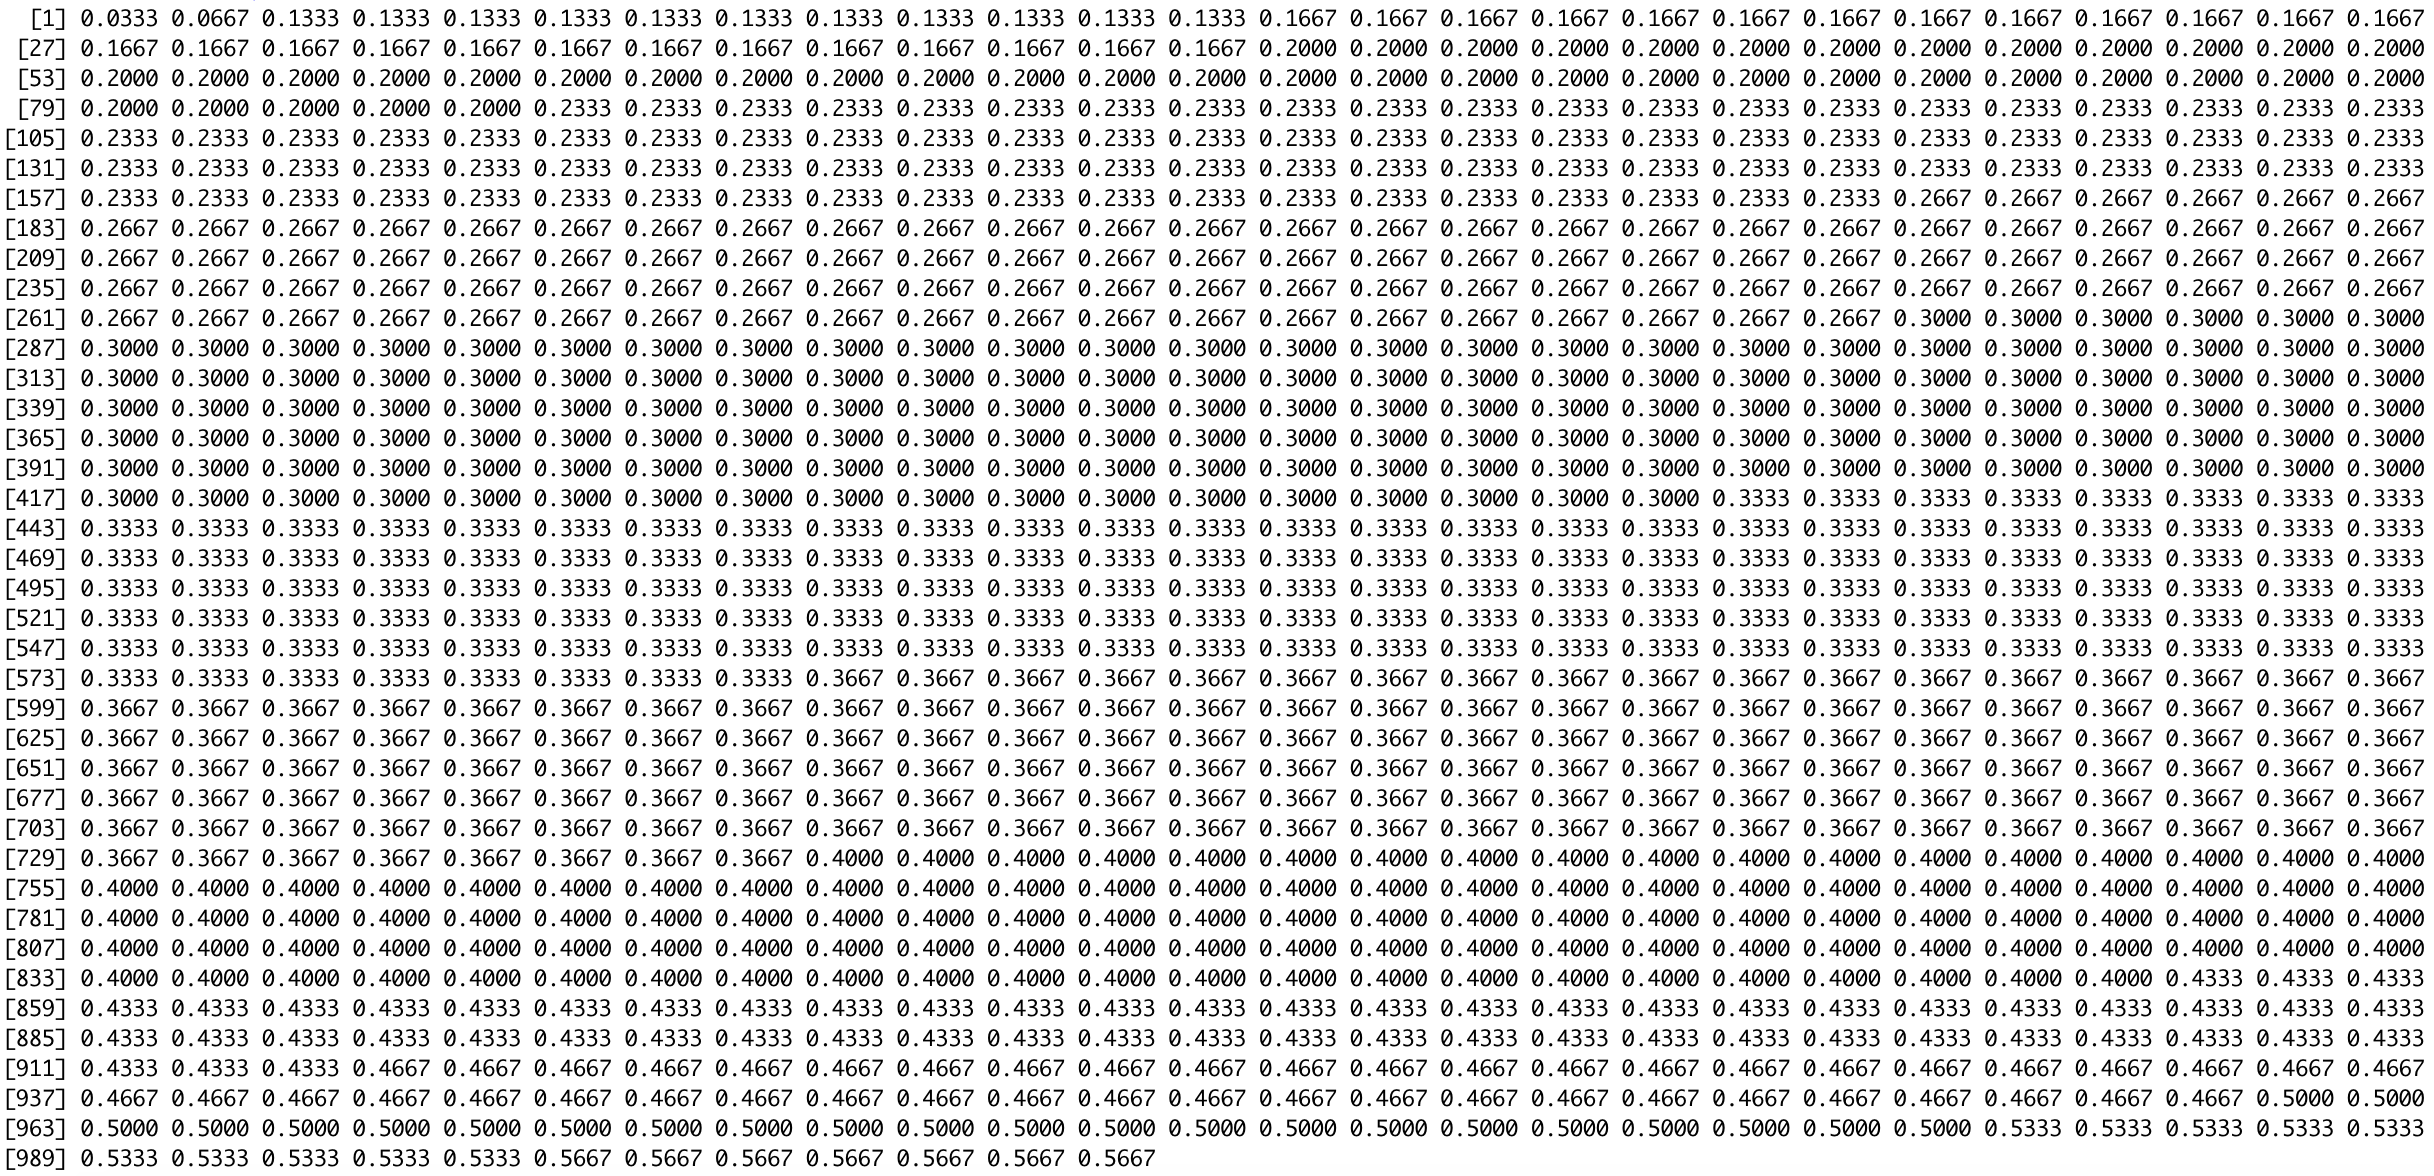
\includegraphics[scale=0.33]{numbers_sorted.png}
\end{center}

\end{frame}

%@@@@@@@@@@@@@@@@@@@@@@@@@@@@@@@@@@@@@@@@@@@@@@@@@
\begin{frame}
\frametitle{Step 3: take the 25th and 975th -- $[0.1667,0.5]$}

\begin{center}
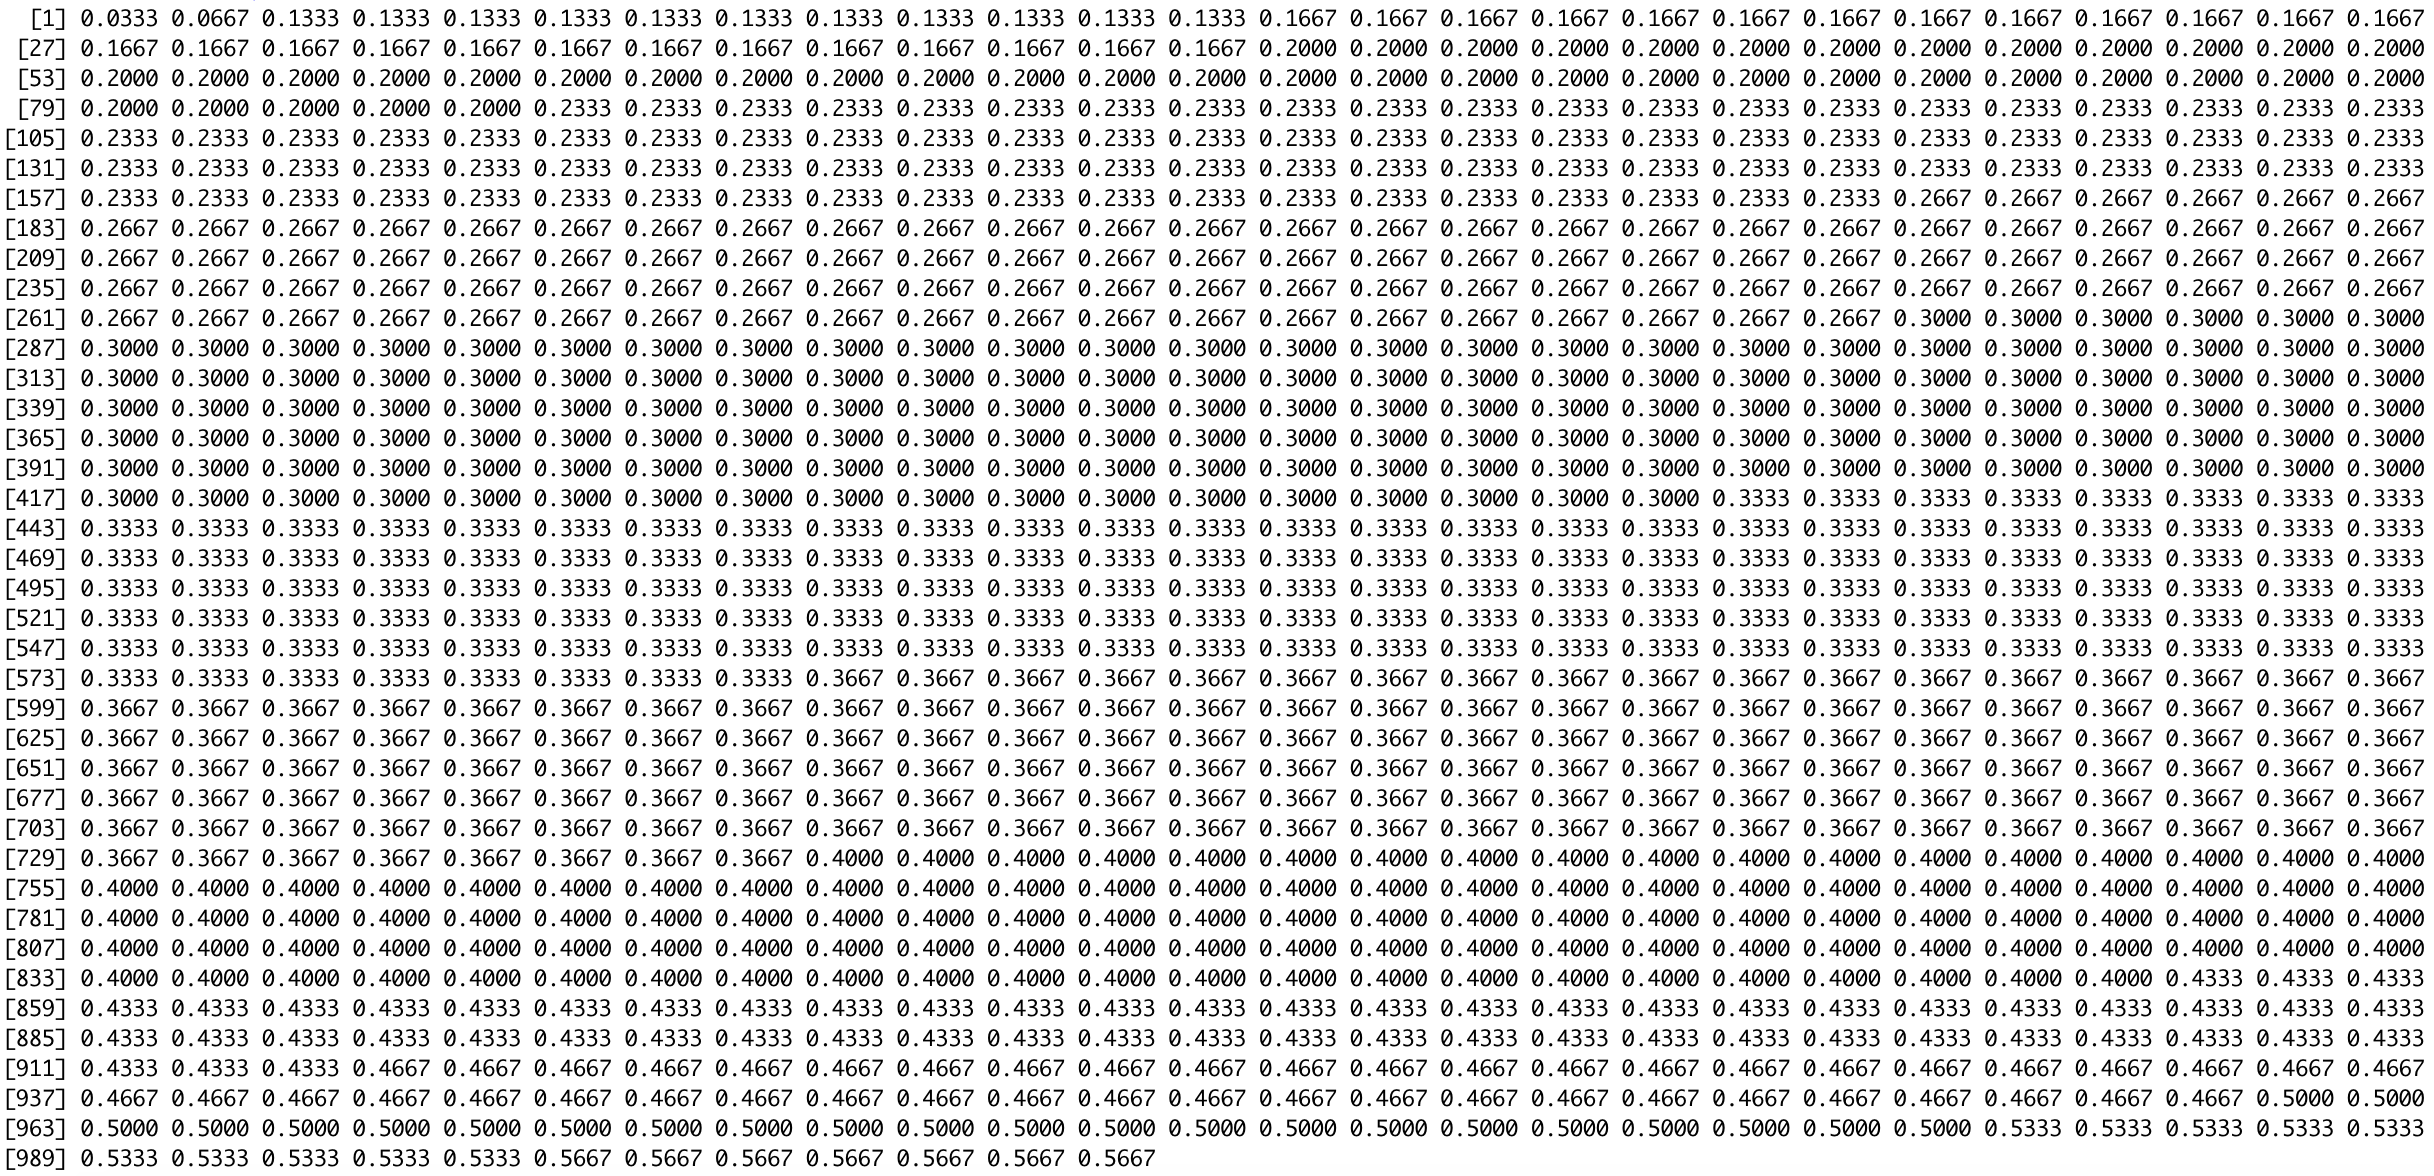
\includegraphics[scale=0.33]{numbers_sorted.png}
\end{center}

\end{frame}

%@@@@@@@@@@@@@@@@@@@@@@@@@@@@@@@@@@@@@@@@@@@@@@@@@
\begin{frame}

\begin{center}
\Huge\textbf{Why should we care?}\\
\bigskip
\bigskip
\large Bootstrapping is a powerful--and pretty easy--way to make robust inferences.\\
\end{center}

\end{frame}



\end{document}
